\documentclass[11pt]{article}
\usepackage[margin=1in]{geometry}
\usepackage{graphicx}
\usepackage{booktabs}
\usepackage{float}
\title{O2 Data Efficiency Report}
\author{Seismic-FNO Experiments}
\date{2026-06-05}
\begin{document}
\maketitle

\section*{Protocol}
The O2 study keeps the fixed 474-GM test set from O1 unchanged and prunes only
the supervised train/validation pool. FNO-Large, Transformer, and BiLSTM are
trained with the O1-final hyperparameters. E-Base is imported from O1 full-data
results.

\section*{Key Conclusions}
\begin{itemize}
\item FNO-Large: E-Base MSE=0.0449, R2=0.9423; reduced runs pending.
\item Transformer: E-Base MSE=0.0214, R2=0.9725; reduced runs pending.
\item BiLSTM: E-Base MSE=0.0099, R2=0.9872; reduced runs pending.
\end{itemize}

\section*{Figures}
\begin{figure}[H]\centering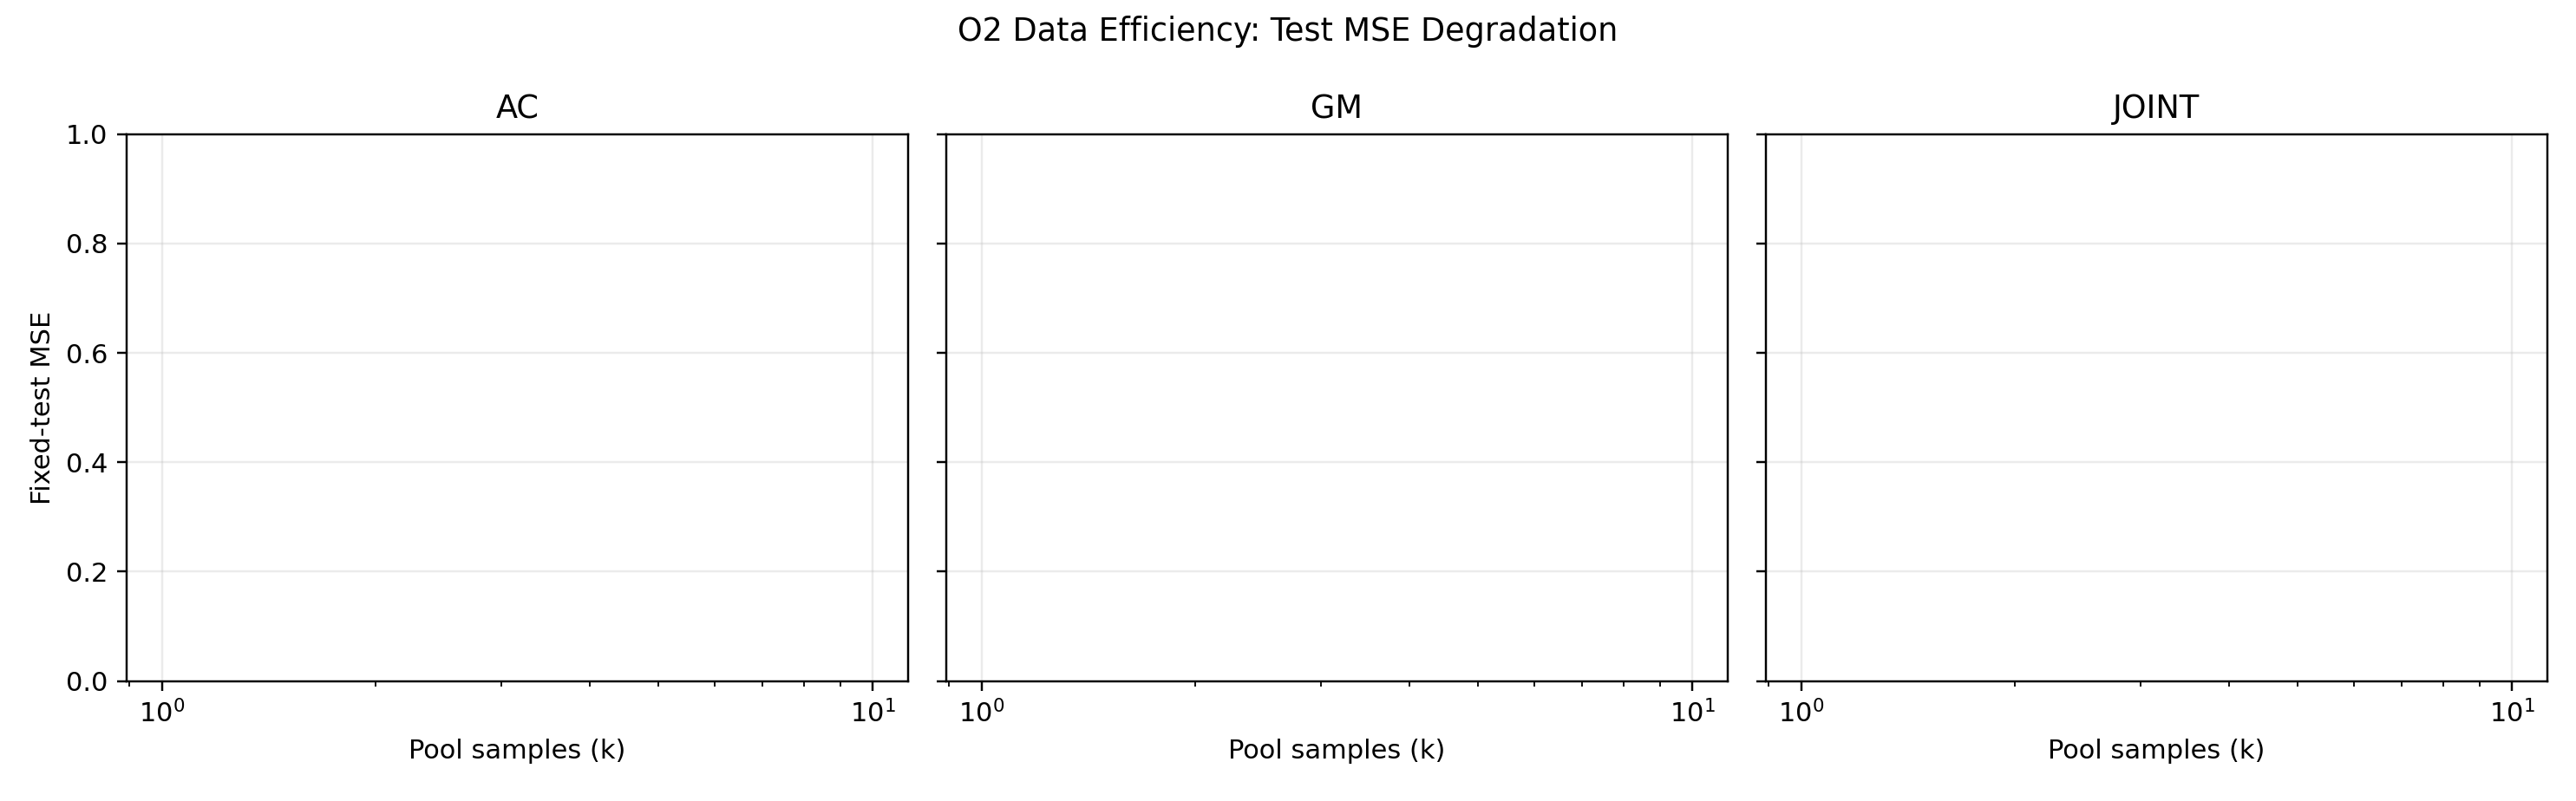
\includegraphics[width=\linewidth]{figures/fig1_mse_degradation.png}\caption{Test MSE degradation.}\end{figure}
\begin{figure}[H]\centering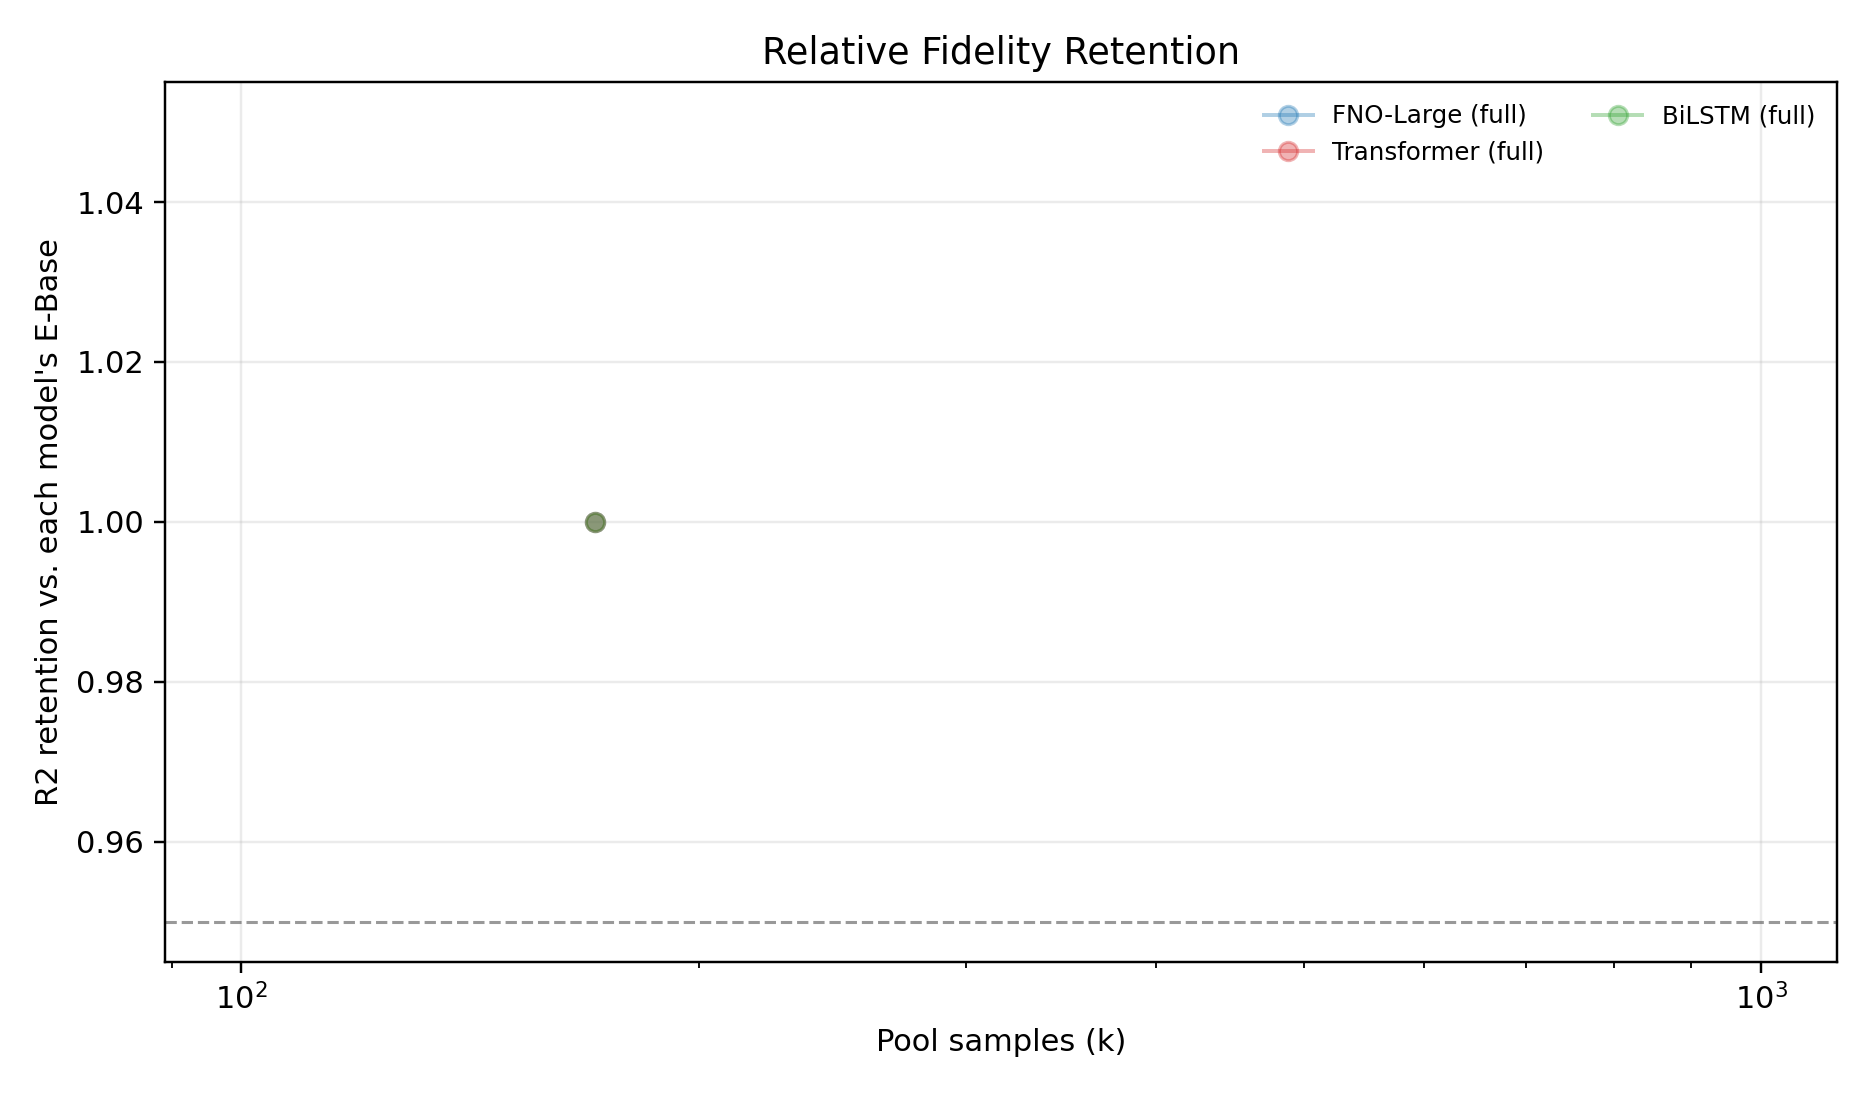
\includegraphics[width=\linewidth]{figures/fig2_r2_retention.png}\caption{R2 retention relative to each model's E-Base.}\end{figure}
\begin{figure}[H]\centering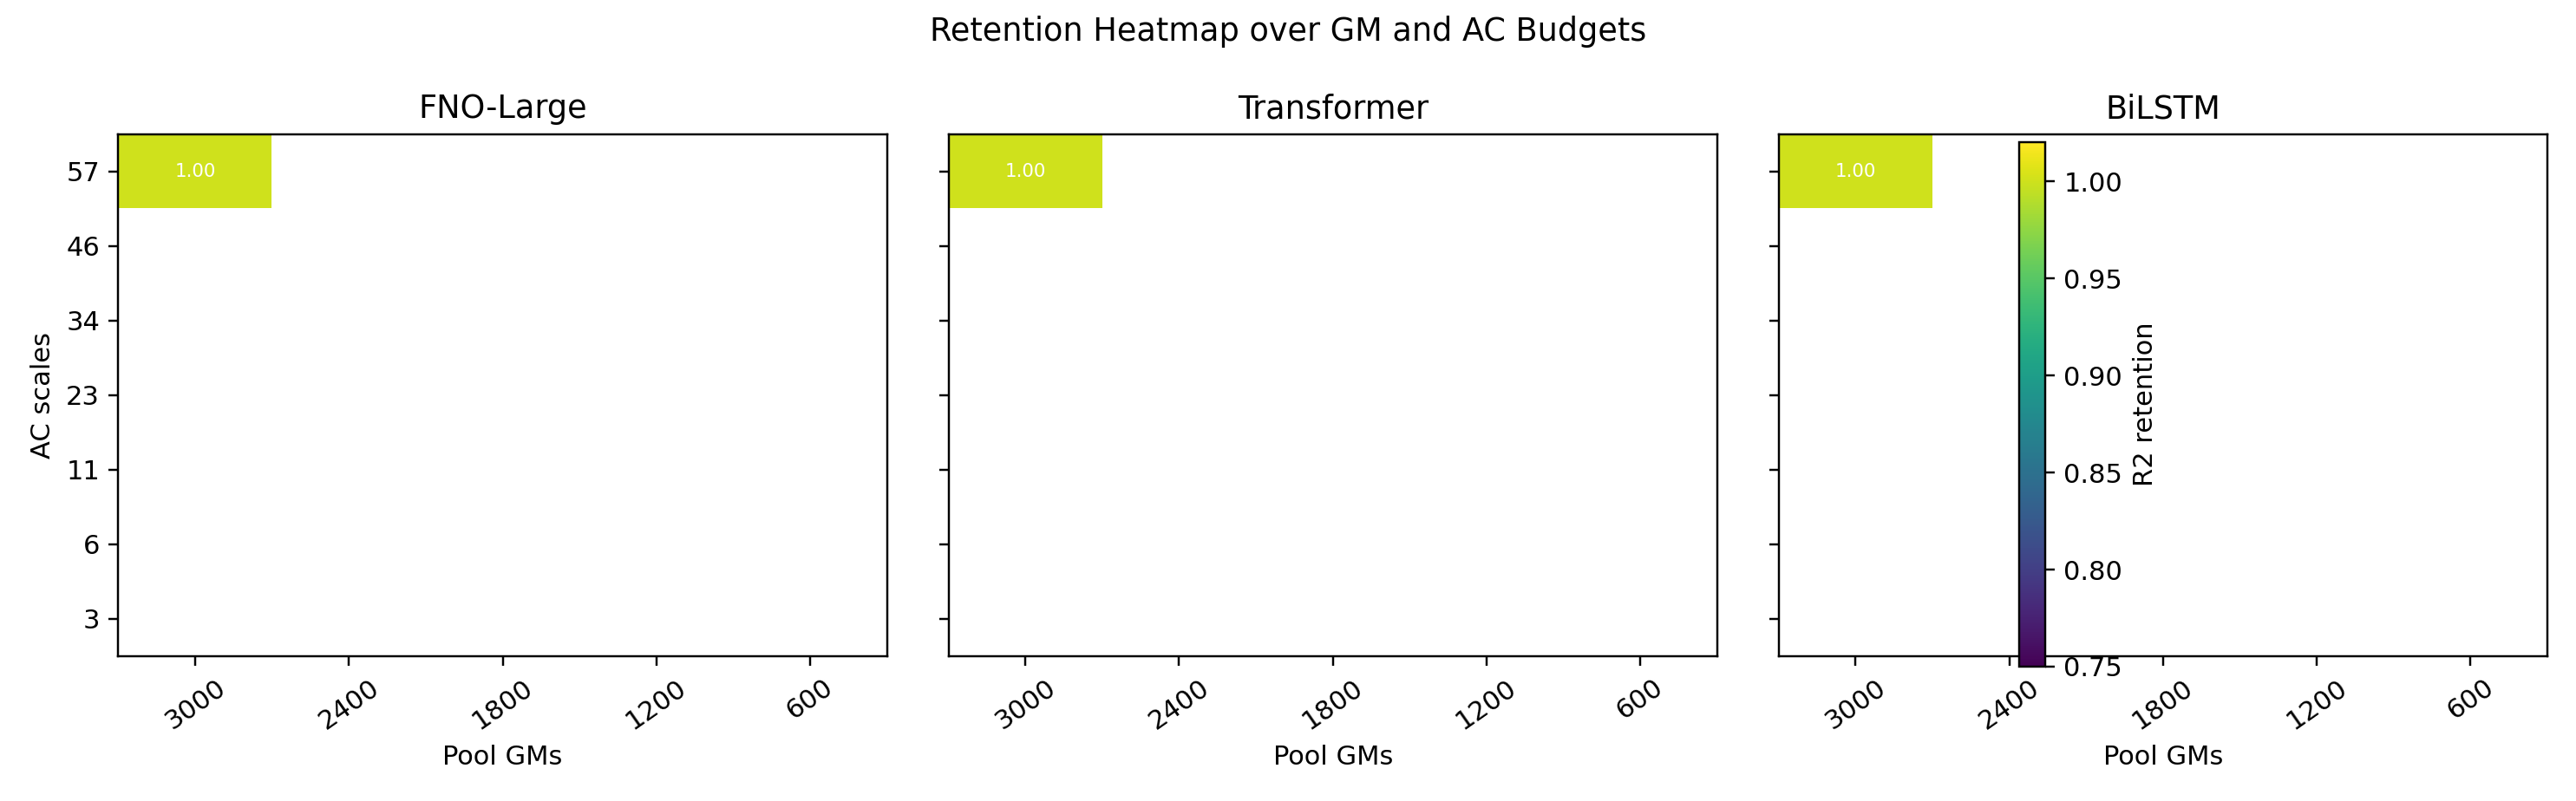
\includegraphics[width=\linewidth]{figures/fig3_retention_heatmap.png}\caption{Retention heatmap over GM and AC budgets.}\end{figure}
\begin{figure}[H]\centering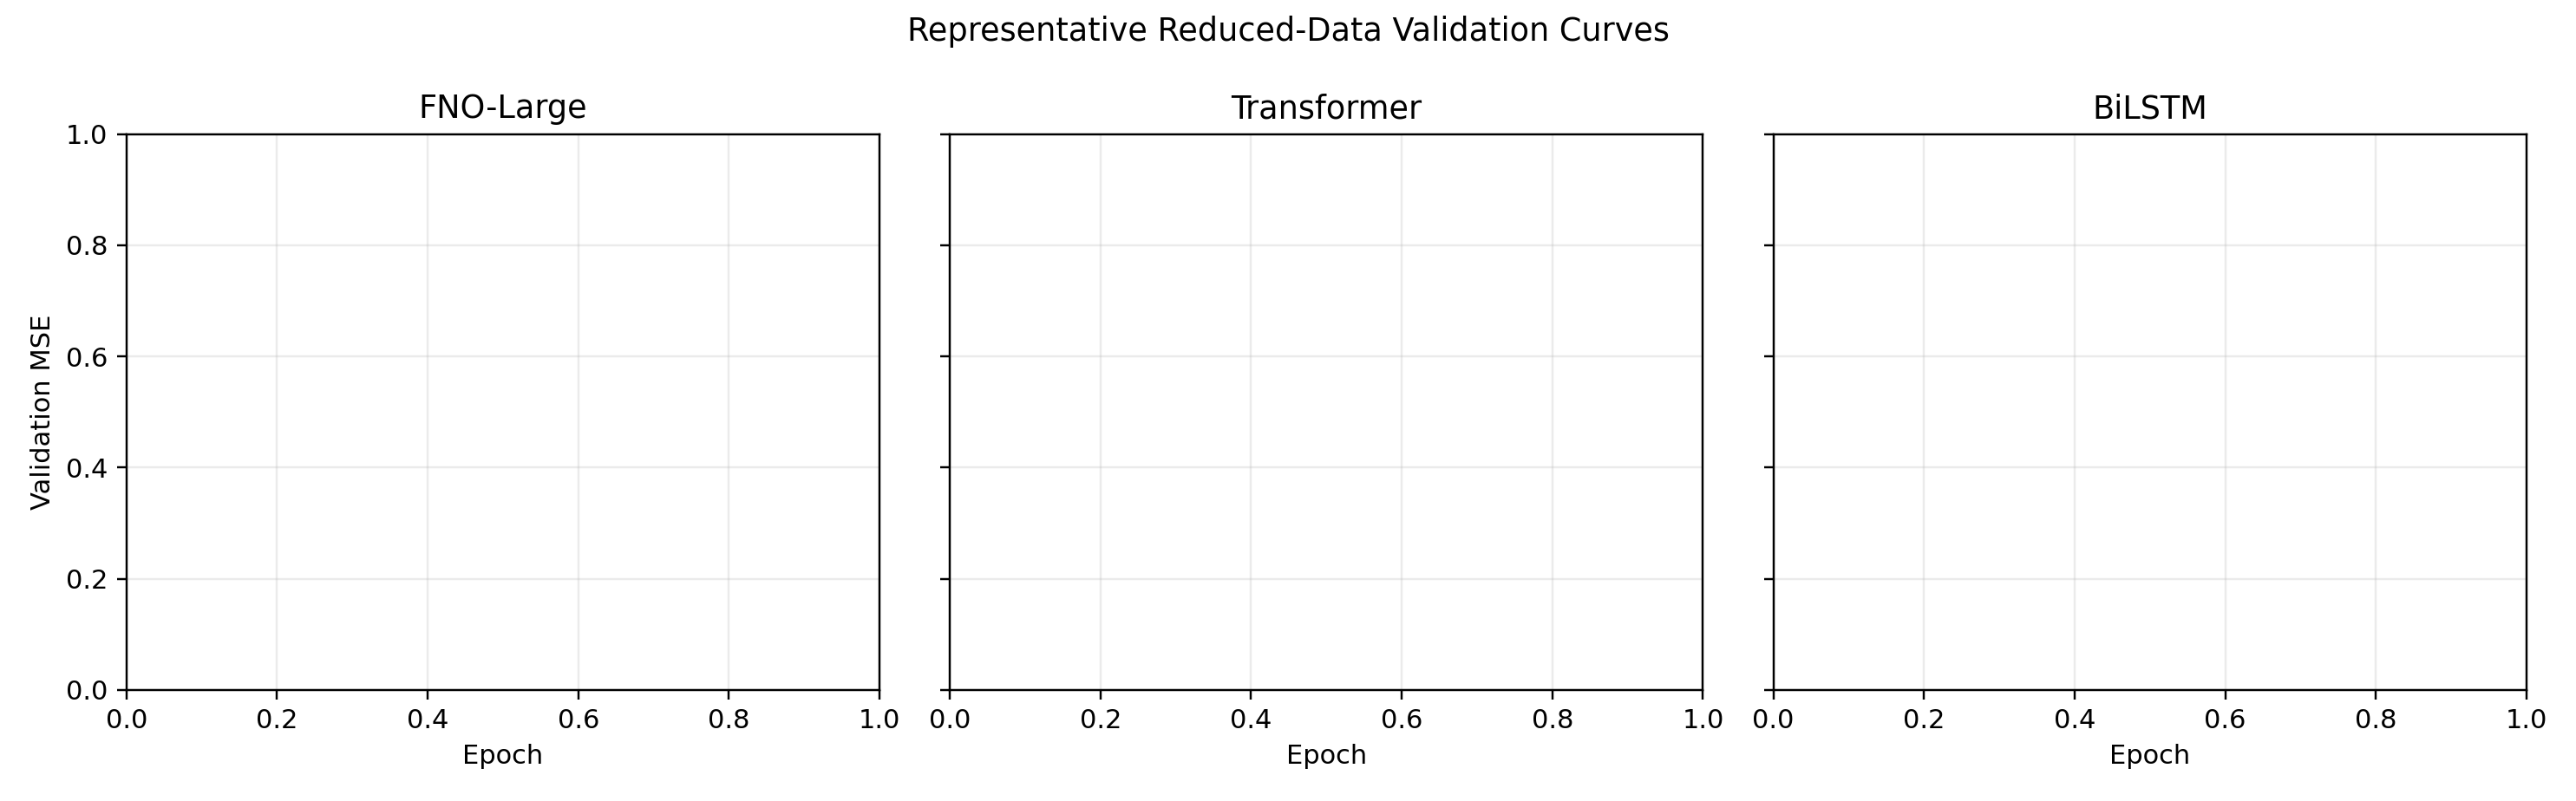
\includegraphics[width=\linewidth]{figures/fig4_training_curves.png}\caption{Representative validation curves.}\end{figure}

\section*{Quantitative Table}
\small
\begin{tabular}{llrrrrrr}
\toprule
Model & Run & GMs & ACs & Pool & MSE & $R^2$ & $R^2$ Ret. \\
\midrule
FNO-Large & E-Base & 3000 & 57 & 171.0k & 0.0449 & 0.9423 & 1.0000 \\
Transformer & E-Base & 3000 & 57 & 171.0k & 0.0214 & 0.9725 & 1.0000 \\
BiLSTM & E-Base & 3000 & 57 & 171.0k & 0.0099 & 0.9872 & 1.0000 \\
\bottomrule
\end{tabular}
\end{document}
